% non-convex kite-shaped cross section
\documentclass[tikz,border=1pt]{standalone}
\begin{document}
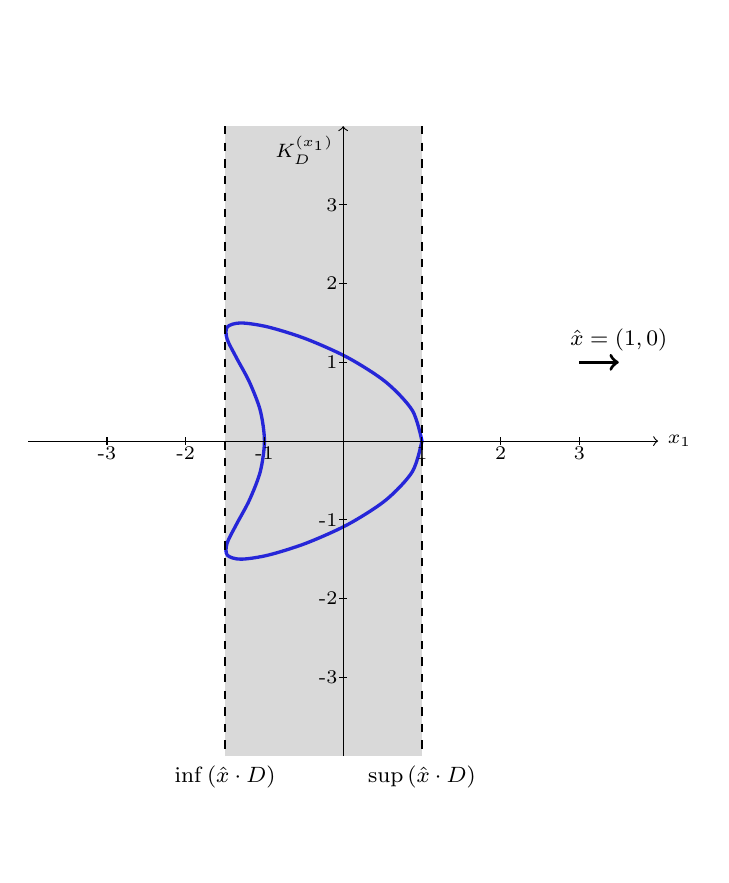
\begin{tikzpicture}
    % kite
    \draw[blue,very thick,domain=0:2*pi,smooth,variable=\t] 
         plot ({cos(\t r) + 0.65*cos(2*\t r) - 0.65},{1.5*sin(\t r)});

    % region
    \draw[line width=2.5cm,color=gray,opacity=0.3] (-0.25,-4) -- (-0.25,4);
    \draw[dashed,thick] (-1.5,4) -- (-1.5,-4) node [below] {\footnotesize$\inf\left(\hat{x} \cdot D\right)$};
    \draw[dashed,thick] (1,4) -- (1,-4) node [below] {\footnotesize$\sup\left(\hat{x} \cdot D\right)$};

    % normal vector
    \draw[very thick,->] (3,1) -- (3.5,1) node [above] {\footnotesize$\hat{x}=\left(1,0\right)$};

    % axis
    \draw[->] (-4,0) -- (4,0) node [right] {\scriptsize$x_{1}$};
    \draw[->] (0,-4) -- (0,4) node [below left] {\scriptsize$K_{D}^{\left(x_{1}\right)}$};

    \foreach \x in {-3,-2,-1,1,2,3}{
        \draw (\x,-0.05) -- (\x,0.05) node [below] {\scriptsize\x};
        \draw (-0.05,\x) -- (0.05,\x) node [left] {\scriptsize\x};
    }    
\end{tikzpicture}
\end{document}